%! Author = adnansiddiquei
%! Date = 05/03/2024

% Preamble
\documentclass[a4paper,11pt]{article}
\pdfoutput=1

% Packages
%\usepackage[colorlinks=true, linkcolor=blue, urlcolor=blue, citecolor=blue, pdfborder={0 0 0}]{hyperref}
\usepackage{url}
\usepackage{jcappub}
\usepackage[T1]{fontenc}
\usepackage{listings}
\usepackage{roboto}
\usepackage{subcaption}
\usepackage{blindtext}
\usepackage{seqsplit}
\usepackage[nottoc]{tocbibind}
\usepackage{siunitx}
\DeclareSIUnit\angstrom{\text {Å}}

%\newcommand{\inlinecode}[1]{\lstinline{#1}}
%\newcommand{\inlinecode}[1]{\texttt{#1}}
\newcommand{\inlinecode}[1]{\texttt{\seqsplit{#1}}}
\lstset{basicstyle=\fontfamily{pcr}\selectfont}


\title{\boldmath Reproducing AstroCLIP: An Evaluation on Cross-Modal Pre-Training for Astronomical Foundation Models}

% %simple case: 2 authors, same institution
\author{Adnan Siddiquei}
\affiliation{University of Cambridge}

% e-mail addresses: one for each author, in the same order as the authors
\emailAdd{as3438@cam.ac.uk}
\note{Word Count: XXXXX (including figure captions and appendix).}


\begin{document}
    \abstract{Lorem ipsum dolor sit amet, consectetur adipiscing elit. Etiam libero purus, lacinia ac nulla id, congue
    dapibus dui. Maecenas gravida ligula a mi tincidunt congue. Cras condimentum tempus leo, vitae aliquam odio consequat
    vel. Pellentesque tincidunt tellus libero, sed cursus mauris sagittis vitae. Integer bibendum metus tellus, vitae
    tempor lectus porta ut. Duis tempus elit id neque aliquam, ac accumsan tellus scelerisque. In at sapien in nulla
    aliquet suscipit ac vel nulla. Suspendisse quis malesuada lacus. Phasellus dapibus sapien dui, vel tincidunt turpis
    convallis eget. Fusce ipsum arcu, pretium nec dui sit amet, viverra interdum lacus. Donec placerat tellus a felis
    sollicitudin, ac egestas leo interdum. Cras facilisis aliquam tortor, ac feugiat nulla dignissim ut.}

    \maketitle
    \flushbottom


    %! Author = adnansiddiquei
%! Date = 04/06/2024

\section{Introduction}\label{sec:introduction}
The size of scientific datasets, particularly in the field of astronomy, has been growing at an ever increasing rate
over the last couple of decades.
Spectroscopic surveys such as the Sloan Digital Sky Survey (SDSS)~\citep{york2000} and more recently the Dark Energy
Spectroscopic Instrument (DESI)\footnote{https://www.desi.lbl.gov/} have been collating millions of galaxy spectra, while photometric
surveys such as the DESI Legacy Survey~\citep{desilegacy2018} has been imaging large portions of the sky extracting millions
of sources.
These datasets are used for a variety of scientific purposes, from understanding the large scale structure of the universe;
estimating galaxy properties such as redshift, stellar mass, and star formation rate; to identifying rare objects such as
quasars and supernovae; and many more.
However, the growing data set size and diversity makes much of this difficult and traditional methods are often
limited by the quality of the data and its associated labels.
One such example is morphological classification, a decade ago we had crowdsourced campaigns such as Galaxy Zoo 2~\citep{willet2013}
which classified approximately 300,000 galaxies, we now have tools such as Tractor\footnote{https://github.com/dstndstn/tractor}
which can probabilistically identify sources from photometric surveys and infer properties such as morphological classification.

More recently, given the unavailability of high quality labels, unsupervised and self-supervised learning methods have been
gaining popularity to tackle these sorts of tasks.
For example,~\cite{liang2023} train a 1D convolutional spectrum autoencoder on spectral data from the DESI Early Data
Release~\citep{desiearly2023} Bright Galaxy Survey for the purposes of outlier detection.
Similarly,~\cite{stein2021} train a 2D convolutional image embedder using a self-supervised technique on galaxy images
from the DESI Legacy Survey for the purposes of similarity search.
They use the Moco v2 self-supervised learning framework~\citep{moco2020, mocov22020}, which is a technique to learn image embeddings
by maximising the similarity of the embedding between augmented views of the same image, and minimising the similarity between
the embedding of different images.
~\cite{hayat2021} also use this technique to train a 2D convolutional model to estimate distances to galaxies from their
photometric images, and further show that the learned embeddings can be fine-tuned very effectively for redshift estimation.
They also show two important conclusions, (1) self-supervised pre-training followed by supervised fine-tuning can achieve
the same performance as supervised training from scratch, whilst requiring significantly fewer labels; and (2) fine-tuning
the self-supervised pre-trained model on the entire Main Galaxy Sample of the SDSS outperforms state-of-the-art supervised
learning methods.
These conclusions are not uncommon in the field of machine learning outside of astronomy
(NLP:~\cite{devlin2019, radford2018}; Medical Imaging:~\cite{shin2016}) and demonstrates the power of transfer learning
and the importance of foundation models for astronomical datasets.

However, as of yet most of these self-supervised learning methods have only been applied to a single modality despite
promising results in cross-modal contrastive learning, such as contrastive language-image pre-training CLIP~\citep{radford2021}.
~\cite{astroclip} pioneer on this front by proposing a multi-modal contrastive learning approach to embed galaxy spectra
and galaxy images into a shared low-dimensional latent space, and in this paper we aim to reproduce their results.
Given the multi-modal nature of astronomical datasets, a useful astronomical foundation model should be able to embed
the varying views of the same object effectively into a shared latent space, allowing for in-modal and cross-modal downstream
application through zero-shot or few-shot learning.

    %! Author = adnansiddiquei
%! Date = 04/06/2024

%\section{Original AstroCLIP Paper}\label{sec:original-paper}
%The original AstroCLIP paper~\cite{astroclip} whose results we reproduce in this paper, implemented a multi-modal contrastive
%learning approach to embed galaxy spectra and galaxy images into a shared latent space.
%This implementation utilised a transformer-based spectrum embedder and a convolutional image embedder to project the two
%modalities into a shared 128-dimensional embedding, and further showed that the learned embeddings were well-aligned
%with the physical properties of the galaxies.
%The authors demonstrated that the learned embeddings could be used to make relatively accurate zero-shot predictions on
%redshift and stellar mass of galaxies using k-NN regression.
%For ease of comparison, we provide a brief overview of the implementation details and key results of the original
%AstroCLIP paper.
%
%\paragraph{Data} The galaxy image data used by the authors~\citep{astroclip} was curated from the DESI Legacy Survey Data
%Release 9~\citep{desilegacy2018}, as prepared by~\cite{stein2021}.
%This was cross-referenced to the DESI Early Data Release~\citep{desiearly2023} to obtain the corresponding galaxy spectra,
%and cross-referenced to the PRObabilistic Value-Added Bright Galaxy Survey (PROVABGS) Catalog~\citep{provabgs2021}
%to obtain the redshift and stellar mass labels for the galaxies - yielding a total of 197,976 galaxy spectra and image pairs.
%
%\paragraph{Spectrum Embedder} The authors pre-trained a transformer-based spectrum embedder using a self-supervised mask
%filling task on the galaxy spectra.
%All the weights of this embedder were then frozen and a single cross-attention layer followed by an MLP was added to project
%the spectrum into a 128-dimensional embedding, yielding a total of 362k trainable parameters.
%
%\paragraph{Image Embedder} The pre-trained convolutional image embedder was acquired from~\cite{stein2021}.
%This image embedder had a ResNet-50 architecture and was trained with a self-supervised method on a sample of 3.5 million
%galaxy images (augmented in a variety of ways) from the DESI Legacy Survey~\citep{desilegacy2018} using the MoCo v2
%framework~\citep{moco2020, mocov22020} in order to embed the images into a 128-dimensional space.
%This image embedder had the convolutional layers frozen and yielding a total of 4.5M trainable parameters in the final
%dense layers of the model.
%
%\paragraph{Training} The authors used a contrastive learning approach to learn a shared embedding space for the images
%and spectra.
%A variety of augmentations were applied to the images and spectra and the respective embedders were trained using an
%InfoNCE loss~\citep{oord2019} over 15,000 iterations with a batch size of 512.
%
%\paragraph{Key Results} The authors demonstrated that the embeddings were well-aligned in 2 main ways:
%In-modal and cross-modal similarity searches using cosine similarity showed that two 'cosine similar' galaxies yielded
%similar spectra and images.
%Secondly, zero-shot regression of redshift and stellar mass using k-NN regression on the learned embeddings similarly
%yielded relatively accurate predictions.
%These are both further discussed in XXXXX when we compare the results of our reproduction with the original paper.

    %! Author = adnansiddiquei
%! Date = 04/06/2024

\section{Data}\label{sec:data}
We use the dataset as provided exactly by~\cite{astroclip}, with minor adjustments.
The dataset contains 197,976 galaxy spectra and image pairs, along with their redshift measurements.
The galaxy spectra were taken from the Dark Energy Spectroscopic Instrument (DESI) Early Data Release~\citep{desiearly2023}
and the galaxy images were taken from the DESI Legacy Survey~\citep{desilegacy2018}.
We summarise the key pre-processing steps relating to the data below.

\subsection{DESI Legacy Survey Images}\label{subsec:images}
The galaxy image dataset was curated by~\cite{stein2022} from the DESI Legacy Survey Data Release 9\footnote{https://www.legacysurvey.org/dr9/description/},
we refer the reader to~\cite{stein2022, astroclip} for a more comprehensive overview of the dataset and its curation, but the
key points are summarised here.
These images were taken by 3 different telescopes, with each telescope focusing on a different combination of sky area
and wavelength range, creating a survey of the sky with a sky coverage of 14,000 $deg^{2}$, at a pixel resolution of 0.262 arcseconds,
across the g (green: $4770 \si{\angstrom}$), r (red: $6231 \si{\angstrom}$), and z (infrared: $9134 \si{\angstrom}$) wavelength
bands\footnote{https://skyserver.sdss.org/dr1/en/proj/advanced/color/sdssfilters.asp}.
The Tractor is used to probabilistically identify and infer properties such
as morphological classification of sources within the survey.
This creates a Tractor catalogue of each identified source, and a sweep catalogue is a subset of this information.
~\cite{stein2022} then filter the dataset as follows: they drop any source that were identified as a star in the sweep catalogues
(Tractor identified a best-fit morphological model of point-spread function, which indicates star); and drop any sources
with a z-band magnitude ($mag_{z}$) larger than 20.
Each remaining source is extracted through a 256x256 pixel cut-out centred on the source, in each of the (g, r, z) bands,
yielding a total of 76,446,849 images.
~\cite{astroclip} cross-match this dataset for their corresponding spectra from the DESI Early Data Release~\citep{desiearly2023}
using the targetIDs associated with the sources, to yield a final dataset of 197,976 galaxy spectra and image pairs.

We perform a variety of augmentations on the images including: a random horizontal and vertical shift; random rotation;
random horizontal and vertical flips as well as adding Gaussian noise.
The 256x256 pixel images all cover more sky than the source being analysed, so we follow~\cite{stein2022} in center
cropping the images to the central 96x96 pixels, adverse to the 144x144 cut-out performed by~\cite{astroclip}.
The choice of the 96x96 cut-out as opposed to a 144x144 cut-out is primarily due to the pre-training of our image embedder
as explained in Section~\eqref{subsec:image-embedder}.
The images are then standardised, ensuring that each channel (g, r, z) of each image had a mean
of 0 and a standard deviation of 1.
The Gaussian noise $\mathcal{G}(0, 0.03)$ was added on top of this standardised data such that each channel was noised
proportionately.


\subsection{DESI Early Data Release Spectra}\label{subsec:spectra}
The spectra were extracted from the DESI Early Data Release~\citep{desiearly2023} and only those that were successfully
cross-matched with the galaxy images were kept.
The spectra ranged the wavelength range of $[3600 \si{\angstrom}, 9824 \si{\angstrom}]$, with a resolution of 7781 pixels per spectrum.
As with the image data, the spectra were also standardised individually, to mean 0 and standard deviation 1, and then
noise $(\epsilon_{sp}(\lambda))$ was added in the form of scaled Gaussian noise as given in Equation~\eqref{eq:spectrum-noise}.

\begin{equation}
\label{eq:spectrum-noise}
    \epsilon_{sp}(\lambda) = \gamma \cdot \sigma_{sp}(\lambda) \cdot \mathcal{G}(0, 1)
\end{equation}
where $\epsilon_{sp}(\lambda)$ is the noise added to the spectrum at wavelength $\lambda$, $\gamma$ is a scaling factor
which is the same for all wavelengths, $\sigma_{sp}(\lambda)$ is the standard deviation of the spectrum at wavelength $\lambda$,
and $\mathcal{G}(0, 1)$ is a standard Gaussian random variable.
$\sigma_{sp}(\lambda)$ was computed for the training set such that $\sigma_{sp}(i)$ $(i \in [0, 7781])$ gave the standard
deviation of all spectra measurements at the $i^{th}$ pixel.
This meant that the noise added to the spectra at any given wavelength was proportional to the variance of the spectra
the given wavelength, which complemented the fact that some wavelengths naturally had more variance than others.
Finally, $\gamma$ was set to 0.3.

\subsection{Redshift measurements}\label{subsec:redshift}
The redshift measurements utilised were the catalog-reported measurements and were compiled and provided directly with the
dataset by~\cite{astroclip}.

\subsection{Further Pre-processing}\label{subsec:pre-processing}
The data was pre-processed further to remove outliers and ensure data was sensible to improve training dynamics.
We dropped any galaxies with a redshift outside the range $[0, 0.8]$ and also dropped any galaxies which had every element
in their spectra equal to 0 (given that they were clearly erroneous).
This resulted in removing a further 380 samples from the dataset, leaving a total of 197,596 galaxy spectra and image pairs.
Our redshift range of $[0, 0.8]$ was larger than the range of $[0, 0.6]$ used by~\cite{astroclip} in their final results.

\section{AstroCLIP Implementation}\label{sec:astroclip-implementation}
Our AstroCLIP model was implemented using a pretrained 2D convolutional image embedder courtesy of~\cite{stein2021}
and a pretrained 1D spectrum embedder courtesy of~\cite{liang2023}.
These were placed into our unified AstroCLIP model and then fine-tuned (with all the weights set as trainable) using
contrastive learning under the InfoNCE loss as per Equation~\eqref{eq:infonce}, to learn the shared low-dimensional
embedding space.
Embeddings were projected into a variety of dimensions: (8, 16, 32, 64, 128, 256, 512) to explore the effect of the
dimensionality of the embedding space on the performance of the model, with~\cite{astroclip} using a 512 dimensional
embedding for their final results.
Below we give a brief overview of the pretraining strategies for the image and spectrum embedders, but for a
comprehensive report we refer the reader to the original papers.

\subsection{Image Embedder}\label{subsec:image-embedder}
\cite{stein2021} trained a galaxy image embedder using a self-supervised method for the purposes of image based similarity search.
The image embedder was trained via the MoCo v2 framework~\citep{moco2020, mocov22020} on a sample of 42 million galaxies
from the DESI Legacy Survey Data Release 9~\citep{desilegacy2018}.
The encoder architecture used was a ResNet-50 architecture.
The images underwent a variety of augmentations (galactic extinction, random rotation, blurring, noising) before
being cropped to the central 96x96 pixels.
The loss function used was the same InfoNCE loss we used in our AstroCLIP model as given in Equation~\eqref{eq:infonce},
and the similarity measure used was also the cosine similarity function as given in Equation~\eqref{eq:cosine-similarity}.
Their model yielded very promising results, and we refer the reader to the original paper for a thorough discussion
on the trained model.
The final fully-connected layers of this model contained 3 layers with 2048, 2048 and 128 units respectively.
The final 128 unit layer was adjusted as required to produce the output dimensionality we desired, but otherwise all
weights and biases were initiated as per the pretrained model.
This yielded between 27.7M and 28.8M trainable parameters depending on the output dimensionality of the model.

\cite{astroclip} pre-train a vision transformer model for their image embedder, we refer the reader to the original paper
for a more detailed discussion on the architecture and pre-training strategy for this.

\subsection{Spectrum Embedder}\label{subsec:spectrum-embedder}
\cite{liang2023} trained a galaxy spectrum autoencoder using galaxy spectra from the DESI Early Data Release~\citep{desiearly2023},
focusing primarily on the Bright Galaxy Survey (BGS) (for precise details on the spectral dataset used, see the original paper).
The autoencoder architecture, named SPENDER, was proposed by~\cite{melchior2022} and encoded the spectra into a 6-dimensional
embedding space.
For our AstroCLIP model, we used the encoder part of the SPENDER model which consisted of a series of 1D convolutional layers
followed by a series of fully-connected layers to bring the dimensionality down to 6.
We reduced the fully-connected layers to 3 layers with 256, $D_{-1}$ and $D_{out}$ units respectively, for any desired
output dimensionality $D_{out}$.
The first 2 fully-connected layers in the pre-trained SPENDER encoder originally had a dimensionality of 256 and 128 units
and as such, for $D_{out} \in [8, 16, 32, 64, 128]$, we retained $D_{-1}=128$ and so the weights and biases of the
first 2 fully-connected layer were retained with the output layer being initialised from a Gaussian distribution.
For $D_{out} \in [256, 512]$, $D_{-1}$ was set to 256 and the entire fully-connected part of the model was retrained
from Gaussian initialisation.
The convolutional layers were initialised from the pre-trained weights of the SPENDER model.
This yielded between 3.1M to 3.3M trainable parameters, depending on the output dimensionality of the model.

\cite{astroclip} once again use a transformer architecture for their spectrum encoder, and we refer the reader to the original
paper for a more detailed discussion on the architecture and pre-training strategy for this.

\section{Model Training}\label{sec:training}
\begin{figure}[t]
    \centering
    \makebox[\textwidth]{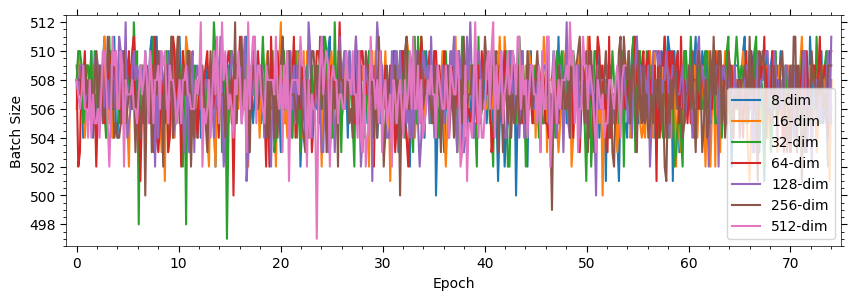
\includegraphics[width=0.9\textwidth]{figures/train_batch_size}}
    \caption{The batch size for each batch after the pre-processing steps were applied to the batch on the fly.
    Each line represents the batch size throughout the training of AstroCLIP models with everything identical except the
    embedding dimensionality.
    The individual lines are not meant to be discernable from one another, but rather this figure should show the general trend.}
    \label{fig:train_batch_size}
\end{figure}

\begin{figure}[t]
\centering
\begin{subfigure}{1\textwidth}
  \centering
  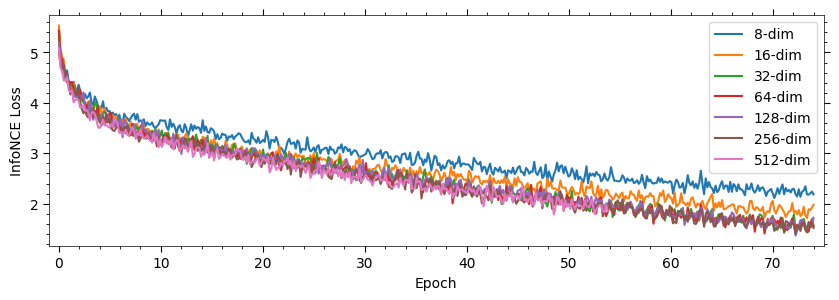
\includegraphics[width=0.9\linewidth]{figures/train_loss}
  \caption{Training loss.}
  \label{fig:train_loss}
\end{subfigure}%
\hfill
\begin{subfigure}{1\textwidth}
  \centering
  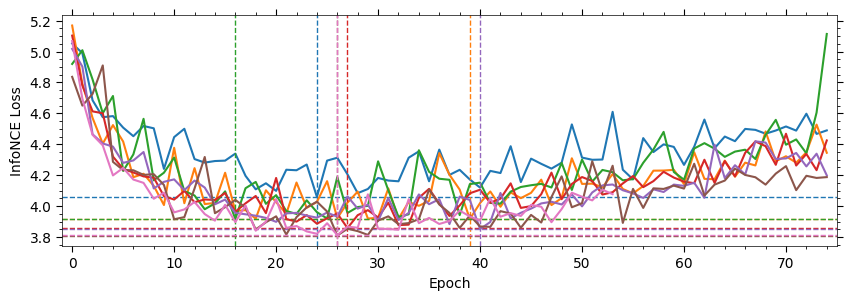
\includegraphics[width=0.9\linewidth]{figures/val_loss}
  \caption{Validation loss.
  The vertical lines correspond to the epoch at which the lowest validation loss was achieved and the horizontal
  line corresponds to the loss value at that epoch.
  The (embedding dimensionality, lowest validation loss, epoch) values are as follows: (8, 4.06, 24); (16, 3.92, 39);
  (32, 3.92, 16); (64, 3.86, 27); (128, 3.85, 40); (256, 3.81, 26); (512, 3.81, 26).}
  \label{fig:val_loss}
\end{subfigure}
\caption{Train and validation loss for AstroCLIP models with varying embedding dimensionality.
The legend on Figure~\eqref{fig:train_loss} applies to both plots.}
\label{fig:train_val_loss}
\end{figure}

Our AstroCLIP model unifies these two embedders into a single model, and then fine-tunes the embeddings using the InfoNCE loss
(Equation~\eqref{eq:infonce}).
The embedding dimensionality was varied through the range $[8, 16, 32, 64, 128, 256, 512]$ and each model was trained for
75 epochs.
Through some exploratory analysis, we fixed a few hyperparameters: batch size of 512; learning rate of $5e^{-4}$; a weight
decay of $1e^{-4}$; and a temperature parameter in the InfoNCE loss of 0.07; and only varied the embedding dimensionality.
One small aspect of note is that the batch size was not consistent throughout training, the pre-processing mentioned in
Section~\eqref{subsec:pre-processing} was performed on the fly on each batch of data as and when randomly sampled by
the DataLoader during training.
This meant that there were small fluctuations in the batch size, and for completeness we show the batch size for each batch
throughout the training of the AstroCLIP models in Figure~\eqref{fig:train_batch_size}.
As can be seen on the figure, the batch size fluctuates very little and generally remains between 502 and 510.
This fluctuating batch size was intentionally left in the training process as it's effects were negligible and would likely
only have a positive effect through the stochasticity it introduces.
The number of epochs required to reach the lowest validation loss, and the corresponding loss is detailed in Figure~\eqref{fig:val_loss}.
Whilst there is a clear pattern in the training loss where the more flexible model appears to be able to achieve the
lowest loss, the same was not true for the validation loss with no clear pattern emerging.
However, it is important to note that a thorough sweep of hyperparameters was not performed, and so it is possible that
a different set of hyperparameters (such as stronger regularisation on the more flexible models, to prevent over-fitting)
could have yielded different results (lower validation loss for the more flexible models).

    %! Author = adnansiddiquei
%! Date = 04/06/2024

\section{Results}\label{sec:results}
To assess and demonstrate the performance of our AstroCLIP model, we reproduce a subset of the downstream tasks from
the original implementation.
The models with the lowest validation loss for each embedding dimensionality (as shown in Figure~\eqref{fig:val_loss})
were selected for evaluation.
The held-out validation set (composing of 39,599 of the 197,976 image-spectra pairs) was used to evaluate the performance
by assessing the accuracy of zero-shot k-NN redshift estimations and qualitative similarity retrieval tasks.
Notation used in this section intentionally follows that of the original paper for the reader's convenience.

\subsection{Zero-shot k-NN Redshift Estimation}\label{subsec:results-redshift-regression}

\begin{figure}[t]
    \centering
    \makebox[\textwidth]{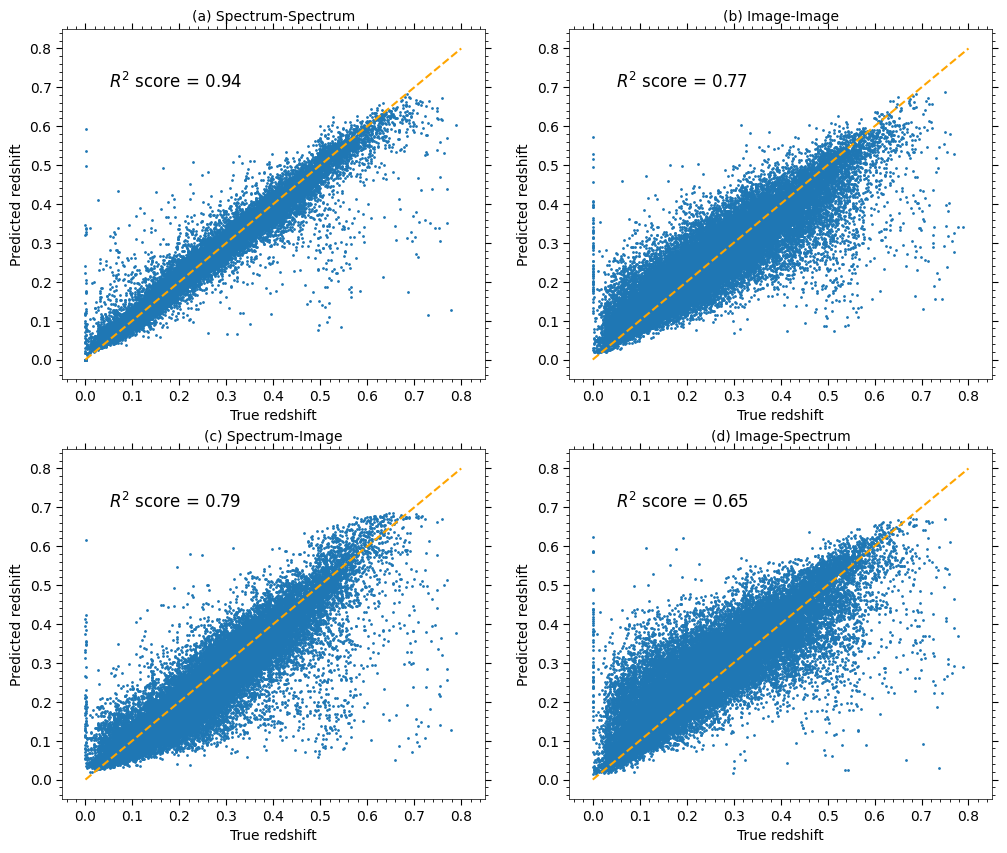
\includegraphics[width=1\textwidth]{figures/redshift_knn_regression}}
    \caption{In-modal and cross-modal zero-shot redshift predictions using k-NN regression on the learned embeddings for the
    best 128-dimensional embedding model.
    The y-axis shows the predicted redshift (the average of the 16 closest neighbours in terms of Euclidean distance) and the x-axis shows the true redshift.
    The dashed line represents a perfect prediction, and the $R^{2}$ of the fit is shown in the top left corner.
    $S_{kNN}(\mathbf{z}_{q}^{sp}, \mathbf{z}^{im})$ indicates the cross-modal prediction where a spectrums redshift was
    predicted using its 16 closes image embedded neighbours.}
    \label{fig:rkr}
\end{figure}

\begin{figure}[t]
    \centering
    \makebox[\textwidth]{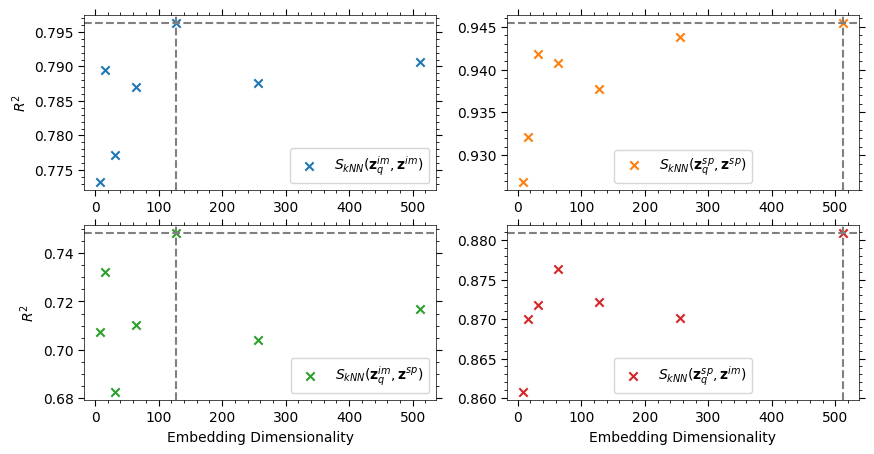
\includegraphics[width=1\textwidth]{figures/r2_vs_embedding_dim}}
    \caption{Exactly the same results as shown in Figure~\eqref{fig:rkr}, but plotted more succinctly for all embedding
    dimensionalities, and all types of in-modal and cross-modal prediction types.
    The dashed lines show the best model for each prediction type.}
    \label{fig:r2_vs_embedding_dim}
\end{figure}

Figure~\eqref{fig:rkr} shows the zero-shot redshift predictions using k-NN regression on the learned embeddings for
the best 128-dimensional embedding model.
Both in-modal (spectrum to spectrum, image to image) and both cross-modal (spectrum to image, image to spectrum)
Figure~\eqref{fig:r2_vs_embedding_dim} then shows this same data in a more succinct manner for all embedding dimensionalities.
These results demonstrate strong evidence that our AstroCLIP model is able to learn a meaningful representation of the
data, as the redshift predictions are highly correlated with the true redshift values, even with low embedding dimensionality.
For a like-by-like comparison to~\cite{astroclip} who use a 512-dimensional embedding, our photometric
$S_{kNN}(\mathbf{z}_{q}^{im}, \mathbf{z}^{im})$ redshift predictions for the 512-dimensional embedding was 0.79 which was
exactly the same as that of~\cite{astroclip}.
However, our spectroscopic $S_{kNN}(\mathbf{z}_{q}^{sp}, \mathbf{z}^{sp})$ redshift predictions for the 512-dimensional
embedding was 0.95 compared to the 0.98 reported by~\cite{astroclip}, which alludes to the effectiveness their novel
transformer architecture for spectral embeddings.
Notably, our 128-dimensional embedding model marginally outperforms the 512-dimensional embedding model in the in-modal
image to image photometric redshift prediction task with an $R^{2}$ value of 0.80, as shown on both Figure~\eqref{fig:rkr}
and Figure~\eqref{fig:r2_vs_embedding_dim}.
This indicates that the vision transformer architecture used by~\cite{astroclip} gave no significant advantage over the
2D convolutional architecture used in this work for the image embedder.
Furthermore, as shown on Figure~\eqref{fig:r2_vs_embedding_dim}, even the low 8-dimensional and 16-dimensional embedding
models perform extremely well across all prediction types, which implies that there is a meaningful amount of mutual
information between the two modalities enabling the model to learn a meaningful representation even in low dimensions.

\subsection{Retrieval by Cosine Similarity}\label{subsec:results-retrieval}
\begin{figure}[t]
    \centering
    \makebox[\textwidth]{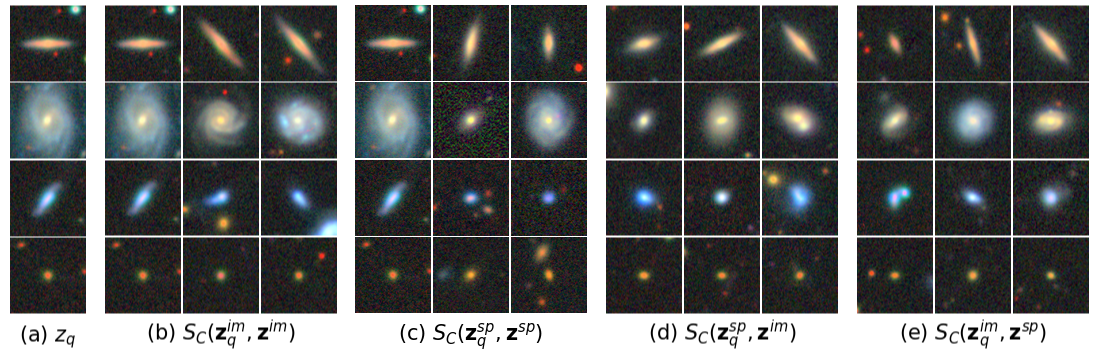
\includegraphics[width=1\textwidth]{figures/sim_search_images_all}}
    \caption{In-modal and cross-modal similarity search using cosine similarity on the learned embeddings for the
        best 128-dimensional embedding model.
        (a) shows the query galaxies; (b) shows the 3 most similar galaxies using an in-modal image to image search; and
        so on.
        By construction, the most similar in-modal galaxy to any given galaxy is itself, hence, the first column of images
        in (b) and (c) are identical to the query image in (a).}
    \label{fig:ssia}
\end{figure}

\begin{figure}[t]
    \centering
    \makebox[\textwidth]{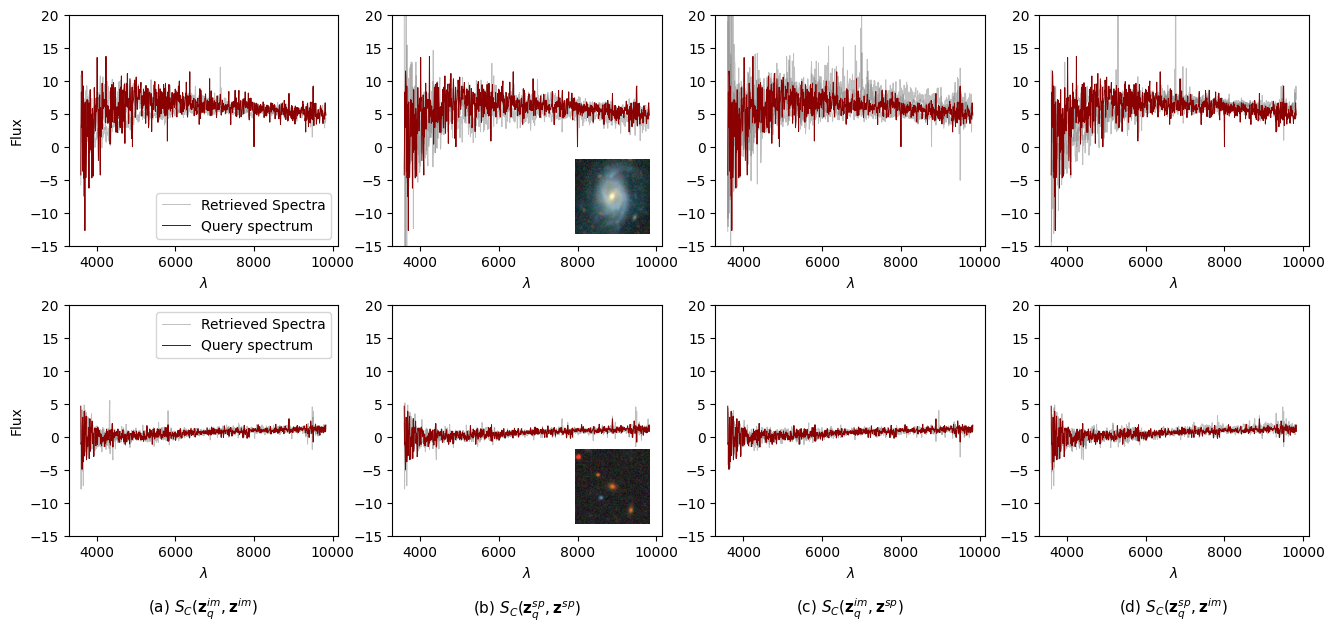
\includegraphics[width=1\textwidth]{figures/sim_search_spectra}}
    \caption{Similar to Figure~\eqref{fig:ssia}, each row in this figure depicts a single query galaxy (query spectrum in red,
        galaxy imaged in plot (b)), with each subfigure showing the spectrum of the 3 most cosine similar galaxies to the
        query galaxy by in-modal and cross-modal similarity search.}
    \label{fig:sss}
\end{figure}

The best 128-dimensional embedding model was used to perform similarity searches using cosine similarity
(Equation~\eqref{eq:cosine-similarity}) on the learned embeddings.
Unlike ~\cite{stein2021}, our model is not constrained to only performing in-modality image searches and Figures~\eqref{fig:ssia}
and~\eqref{fig:sss} show the results of both in-modal and cross-modal similarity searches for images and spectra respectively.
The results show that the model is able to retrieve similar images and spectra to the query image and spectrum, respectively,
even across modalities.
As described by ~\cite{stein2021}, this ability is critical when searching for rare astronomical sources and the cross-modal
ability of the model adds significantly to this.

    %! Author = adnansiddiquei
%! Date = 28/06/2024

\section{Conclusion}\label{sec:conclusion}
In this report, we present a successful reproduction of the AstroCLIP model by~\cite{astroclip}.
We utilise different architectures for the image and spectrum embedders, but ultimately achieve similar results
and show that the model is able to learn a meaningful representation of the data.
We also explore the effect of different embedding dimensionalities on the performance of the model and show that
even low-dimensional embeddings are able to capture a meaningful amount of mutual information between the two modalities,
given their strong performance in the zero-shot redshift prediction tasks.
Our results do bring into question the optimal architecture for the image embedder and the minimum required
embedding dimensionality, as our 128-dimensional model marginally outperforms the 512-dimensional model by~\cite{astroclip}
in the in-modal image to image redshift prediction task.
Nonetheless, our results alongside those of~\cite{astroclip} demonstrate that it is possible to achieve high quality foundation
models for astronomical data using cross-modal contrastive pre-training, and that the learned embeddings can be used for a variety
of downstream tasks with strong performance.
This has a variety of impacts on the field of astronomy, such as enabling cross-modal similarity searches for rare or interesting
objects, and enabling the use of pre-trained foundation models for transfer learning on smaller datasets for specific tasks.


    \clearpage

%    \nocite{*}
    \bibliographystyle{apalike}
    \bibliography{main}
    \clearpage

    %\appendix

    %\section{Appendix A}\label{app:app-a}
    %Lorem ipsum dolor sit amet, consectetur adipiscing elit. Suspendisse eget urna laoreet, elementum tellus nec, dapibus dui.
\end{document}
